\cotefile{157-4}
\scanpage{379}
\mspage{\unsure{153|103}}
% archive sheet number: 378
flèches de la forme $f\times\mathrm{id}_X:S\times X\longrightarrow T\times X$, où $f:S\unsure{\relbar|\longrightarrow}T$ est un morphisme entre ensembles ordonnés finis. Ou plus généralement, entre ensembles ordonnés $S,T$ tels que $S^{\unsure{o|0}}$ soit artinien, \unsure{i.e.} $S$ noethérien, et que $\mathrm{Esp}(S^o)$ soit noethérien. Cette dernière hypothèse étant inutile sous l'axiome $\mathrm{Loc}(8)$ \unsure{des limites|en limite}, cf $\underline{\overline{\mathrm{XVII}}}$ th.~3.1 p.~56.) Donc ce n'est pas encore le résultat rêvé !

7.5. Le seul cas que je connaisse où $f_*$ existe pour \uline{toute} flèche dans $\mathrm{Cat}$, c'est le cas où $W$ satisfait :
\[
\underline{\mathrm{Loc}(\deleted{\unsure{1\ \mathrm{bis},|1,}}\ 6a,8,9)}\,,
\]
% slanted
\margin{vérifier s'il ne faut pas aussi la condition $\mathrm{Loc}(3\,\mathrm{bis})$ en plus de $\mathrm{Loc}(6a,8,9)$ \unsure{($\alpha$)} Vérification faite, c'est OK \unsure{sans} $\mathrm{Loc}(3\,\mathrm{bis})$}
\margin{\uline{NB} Après nouvelle réflexion, il \unsure{apparait|apparaît} qu'il suffit même $\mathrm{Loc}(6'a,8,9)$}
c'est à dire \deleted{l'axiome $W=W^{\unsure{(6)|6}}$ des facteurs directs,} l'axiome des $W$-asphérisations faibles, déjà abondamment mentionné, et enfin \unsure{ceux|aux} des limites et d'accessibilité, i.e. $W$ est \unsure{$L_1$|Lim}-accessible dans $\underline{\mathrm{Fl}}(\mathrm{Cat})$.

Le résultat-clef pertinent est donné dans XV 8.4. (p.~105-\unsure{107|106}), qu'il faut souder à XV 7.4. (p.~98-99) pour en faire
\scanpage{380}
\mspage{104}
% archive sheet number: 379
bon usage, et en déduire le \deleted{\unsure{XV}} Th.~10.1 (XV, p.~134-136). Mieux que l'existence des $f_*$, l'ensemble d'axiomes \unsure{étonnamment} faibles que je viens d'expliciter \unsure{suffit} à assurer que $\mathrm{HOT}_W$ est un \uline{dérivateur} sur $\mathrm{Cat}$ \deleted{\unsure{tout|tous}} \unsure{entier|entière}, au plein sens du terme, i.e. qu'il satisfait à $\mathrm{Der}(1,2,3,\deleted{\unsure{4^*}}4,\deleted{\unsure{5^*}}5,6,4^*,5^*,6^*)$.

Ceci est obtenu en remplaçant \inserted{(grâce à XV 8.4)} $\mathrm{Cat}$ par $A^{\wedge}$, où $A$ est une catégorie-test convenable, \inserted{$W$ par $W_A\subset\mathrm{Fl}\,A^{\wedge}$,} et en prouvant que \deleted{la} \deleted{\unsure{dér}} $\unsure{W_A|W/A}$ s'insère dans un triple de Quillen clos $(W,C,F)$, avec $C=\mathrm{Mono}(A^{\wedge})$, ce qui détermine $F$ comme $(C\cap W_A)_*$. On applique alors $\underline{\overline{\mathrm{XV}}}$ 7.4. à cette situation (résultats résumés dans XIX th.~2.3 (p.~19), 2.6 (p.~25) 2.9 (p.~28).
On retrouve l'existence des $f_!$ (avec un mode de calcul bien différent du \unsure{calcul|celui} dans $\mathrm{Cat}$ !), et en plus on trouve l'existence des $f_*$ (plus l'exactitude des carrés
\scanpage{381}
\mspage{105}
% archive sheet number: 380
des carrés $W$-cartésiens) -- ce qui pour moi, pendant un bon moment, était \uline{le} gros problème pour la théorie de $\mathrm{HOT}_W$ !).

Je trouve époustouflant qu'on parvienne à un résultat aussi fort avec des axiomes aussi \unsure{ridiculement|radicalement} faibles. Plus particulièrement, qu'on ait toutes les propriétés \deleted{de la} désirables de la structure homotopique droite, sans avoir à faire sur $W$ aucune hypothèse du type $W$-fibrations !
Ces axiomes n'impliquent \uline{pas} l'axiome $\mathrm{Loc}(7)$ (équivalent à $\mathrm{Loc}(7\mathrm{D}_{W_{\unsure{\omega|w|\infty}}})$ en présence de $\mathrm{Loc}(8)$), comme on a vu sur l'exemple de $\mathbb{W}_{\unsure{0|o}}$. Impliquent-ils \deleted{\unsure{tout}} au moins $\mathrm{Loc}(7\mathrm{F})$, i.e. l'existence d'assez de $W$-fibrations ? Je ne hasarderais aucune conjecture à ce sujet ! Mais il faut \unsure{bien} se dire qu'en l'absence de $\mathrm{Loc}(7)$ (et même
\scanpage{382}
\mspage{106}
% archive sheet number: 381
en admettant $\mathrm{Loc}(7\mathrm{F})$), tout en sachant que la structure homotopique droite associée à $W$ est parfaite à tous égards, on n'a à priori aucune maîtrise sur celle-ci, notamment pour le calcul des fibres $W$-homotopiques et la construction \unsure{des|de} carrés $W$-cartésiens.

Même en ramenant toutes ces constructions à $A^{\wedge}$ (\unsure{prenant}, \unsure{tant y étant|tant qu'à faire}, $A=\mathbb{\Delta}$, \deleted{\unsure{)}} i.e. \unsure{se ramenant|en revenant} au contexte semisimplicial), quoiqu'on sache qu'il y a une factorisation \uline{fonctorielle} $f=pi$ avec $\deleted{i\in W_A,\ p\in}\ i\in \mathrm{TC}\subset W_A$, $p\in F\subset\mathrm{Fib}_{W_A}$, je ne vois aucune façon concrète de l'expliciter.
À moins que la considération des chemins infinis, qui (en l'absence de $\mathrm{Loc}(7)$) \unsure{s'avèrent|s'avère} \unsure{inopérants|inopérante} dans $\mathrm{Cat}$, \unsure{sauve|s'avère|s'avérer} \unsure{la mise|là utile} dans $\mathbb{\Delta}^{\wedge}$ ??

\scanpage{383}
\mspage{\unsure{157|107}}
% archive sheet number: 382
Question qui devrait être facile à élucider, mais sur laquelle je ne veux pas m'attarder à présent.

Notons en passant que le résultat de saturation forte de Quillen, pour les triples de Quillen clos, montre que l'ensemble d'axiomes $(\unsure{*|\bullet})$ implique \deleted{que} l'axiome $\mathrm{Loc}(\unsure{1\mathrm{ter}|M\mathrm{ter}})$, i.e. que $W$ est \uline{fortement saturé}.

Notons aussi que contrairement à ce qui a lieu pour les $f_!$, je ne sais prouver l'existence de $f_*$, et notamment des suites de cosuspension, que sous des conditions \inserted{(soit $\mathrm{Loc}(7\mathrm{D}_{W_{\unsure{\omega|w|\infty}}})$, soit $\mathrm{Loc}(6a,8,9)$)} qui assurent déjà que les carrés $W$-cartésiens sont exacts, et par suite les suites de cosuspension exactes.
\figure{\begin{tikzpicture}\draw (0,0) -- (.30,-.24);\end{tikzpicture}}

Je pense que dans \unsure{les} pages précédentes j'ai dit tout ce que je sais dire de pertinent, concernant les questions 1, 2, 4 soulevées \unsure{dans|en} 7.1. Ces réponses me parais%
\scanpage{384}%
\mspage{108}%
% archive sheet number: 383
sent satisfaisantes -- plus \unsure{satisfaisante|satisfaisantes} que je ne l'aurais osé espérer pendant les premiers deux mois de mes cogitations ! Il reste les questions 3 et \unsure{1bis}, que je vais à présent examiner.
% slanted
\margin{Pour les axiomes $\mathrm{Der}(1)$ à $\mathrm{Der}(6^*)$, cf I p 67-68. Les axiomes $\mathrm{Der}(6,6^*)$ sont les axiomes ``de Heller'' dont la nécessité m'est apparue \unsure{seulement} ultérieurement.}

7.6. \unsure{Soit|Soient} les différents axiomes des localiseurs : sous quelles conditions sur $W$ \unsure{un|chacun} de ces axiomes est-il satisfait \unsure{pour} $\mathrm{HOT}_W$ ? Pour ce qui est des axiomes $\mathrm{Der}(4,5,6,4^*,5^*,6^*)$, je crois avoir dit tout ce que je sais en dire, et avoir des critères de validité parfaitement maniables, dans les pages précédentes. Résumons pourtant :
\inserted{Structure \unsure{à|:} cofibr. : $\mathrm{Loc}(6a)$ ($+\mathrm{Loc}(3\,\mathrm{bis})$?}
\inserted{Structure à fibrations : $\mathrm{Loc}(7\mathrm{D}_{W_{\unsure{\omega|w|\infty}}})$}
\diagram{\(\displaystyle
\left\{
\begin{array}{@{}l@{}}
\left.
\begin{array}{ll}
\mathrm{Der}(4^*,5^*): & \underline{\mathrm{Loc}(3\,\mathrm{bis})}\ \deleted{\unsure{6}}\\
\mathrm{Der}(4^*,5^*,6^*): & \underline{\mathrm{Loc}(3\,\mathrm{bis},6a)}
\end{array}
\right|\quad \text{ou }\mathrm{Loc}(6'a,8,9)\\
\mathrm{Der}(4,5,6)\ \inserted{\text{(sur Cat)}}\ \text{(et \unsure{tout le reste|tous les vents} !)}:
\quad\underline{\mathrm{Loc}(6'a,8,9)}\\
\mathrm{Der}(4,5,6)\ \text{sur }\mathrm{Diag}=\text{ens.}\qquad:
\quad\underline{\mathrm{Loc}(7\mathrm{D}_{W_\omega})}\ \text{(ou}\\
\hspace{6em}\text{ordonnés finis}\hspace{7em}\text{seulement }\mathrm{Loc}(7\mathrm{F})\text{)}
\end{array}\right.
\)}

Il reste les axiomes $\mathrm{Der}\,1$ (décomposition) $\mathrm{Der}\,2$ (localisation) $\mathrm{Der}\,3$ (objet unité), que je vais passer à présent en revue. On vérifie
\scanpage{385}
\mspage{109}
% archive sheet number: 384
de façon quasi-tautologique que l'axiome $\mathrm{Der}\,1$ est satisfait sans condition sur $W$ (pas même $\mathrm{Loc}(2,3)$ !) -- en fait, il est satisfait pour \unsure{tt} prédérivateur $D_{(M,W)}$ défini par une catégorie de modèles.

L'axiome de localisation $\mathrm{Der}(2)$ est par contre \deleted{nettement plus} \inserted{de nature} délicate. \deleted{\unsure{Je ne}} Il est valable, plus généralement, pour une catégorie de modèles $(M,W)$ (définissant \inserted{un prédérivateur} $\mathbb{D}=\mathbb{D}_{(M,W)}$) et un objet $S$ de $\mathrm{Cat}$, lorsque $(M(S),W(S))$ est associé à une structure à fibrations ou à cofibrations, ce qui par K.~S.~Brown implique que \unsure{tte} \unsure{flèches|flèche} de ${\mathrm{H}\unsure{\mathrm{O}|\mathrm{o}}\deleted{\unsure{\mathrm{T}}}}_W(S) =M(S)W(S)^{-1}$ se ``réalise'' par une flèche de $M(S)$ -- et alors le résultat est évident. La condition que je viens de dire est satisfaite \deleted{\unsure{sous les deux|sur les deux}} \inserted{lorsque} \deleted{\unsure{axi}} $(M,W)$ lui-\ensuremath{=} est associé à une structure de cofibrations ou de fibrations,
\scanpage{386}
\mspage{110}
% archive sheet number: 385
et si de plus on suppose que l'on est dans l'un des deux cas suivants

a) $S$ est un ens. ordonné fini (ce qui nous amène à nous restreindre, à défaut de mieux, à $\mathrm{Diag}={}$\unsure{ss}-catégorie de $\mathrm{Cat}$ formée des ens. ord finis).

b) La factorisation stipulée dans l'axiome de factorisation $f=pi$ [avec $i\in\mathrm{Cof}$, $p\in W$ (cas des cofibrations) ou $i\in W$, $p\in\mathrm{Fib}$ (cas des fibrations) peut-être choisie fonctorielle en $f$.

Or, dans le cas de $\mathrm{Cat}$, dans les cas où on sait prouver que $W$ est associé à une structure à cofibrations (axiome $\underline{\mathrm{Loc}(6a)}$) ou à fibrations (axiome $\underline{\mathrm{Loc}(7\mathrm{D}_{W_{\unsure{\omega|w|\infty}}})}$), on trouve bel et bien une factorisation fonctorielle. Donc chacun de ces axiomes\unsure{,} \deleted{ainsi} implique $\mathrm{Der}\,2$\unsure{:|.}

\scanpage{387}
\mspage{111}
% archive sheet number: 386
\figure{\makebox[\linewidth][l]{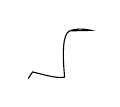
\begin{tikzpicture}[x=.55cm,y=.55cm]
\draw (0,0) -- (.1,.15) .. controls (.4,.08) and (.63,0) .. (.84,.03)
.. controls (.79,.57) and (.79,1.03) .. (.96,1.10)
.. controls (1.10,1.16) and (1.34,1.14) .. (1.45,1.11)
-- (.98,1.10);
\end{tikzpicture}}}
Reste l'axiome de \deleted{l'objet final}\inserted{contractibilité} : si $S$ dans $\mathrm{Cat}$ \deleted{a un objet final}\inserted{est \unsure{contractible|contractile}}, est-il $\mathrm{HOT}_W$-asphérique i.e. le foncteur
\[
\mathrm{HOT}_W(e)=\mathrm{Hot}_W\unsure{\relbar|\longrightarrow}\mathrm{HOT}_W(S)
\]
est-il pleinement fidèle ? Quand on dispose \deleted{de $\mathrm{Loc}(\unsure{3}$} de la théorie des $f_!$ ``\deleted{\unsure{dans}}\unsure{via|sur} $\mathrm{Cat}$'' (donc sous le seul axiome $\underline{\mathrm{Loc}(3\,\mathrm{bis})}$, on trouve ceci (noté dans $\underline{\overline{\mathrm{VI}}}$ p.~\unsure{202|252}) :
% slanted
\margin{moyennant $\mathrm{Loc}(3\,\mathrm{bis})$}

Soit $f:\unsure{\mathbb{S}|S}\to T$ une flèche de $\mathrm{Cat}$. Pour que ce soit une $\mathrm{HOT}_W$-équivalence, i.e. pour que $f^{\unsure{*|\wedge}}:\mathrm{HOT}_W(T)\to\mathrm{HOT}_W(S)$ induise un foncteur \uline{pleinement fidèle} sur la sous-catégorie des objets constants de $\mathrm{HOT}_W(T)$, il f. et s. que $\mathrm{hot}_W(f):\mathrm{hot}_W(S)\longrightarrow\mathrm{hot}_W(T)$ soit \unsure{iso.} Donc il \uline{suffit} que $f\in W$, et cette condition est aussi nécessaire si $\deleted{\unsure{g|S}}W$ est \deleted{fortement} saturé (axiome $\mathrm{Loc}(1\,\unsure{\mathrm{bis}|\mathrm{ter}})$).

Par acquit de conscience, j'explicite ici la démonstration. L'existence des foncteurs
\scanpage{388}
\mspage{112}
% archive sheet number: 387
$f_!$, en particulier des objets d'homologie $H_{\unsure{\bullet|0}}^{\mathrm{HOT}_W}(S,\unsure{\xi|\zeta})$ (ou simplement $H_{\bullet}^W(S,\xi)$) pour $\xi\in\mathrm{HOT}_W(e)=\mathrm{Hot}_W$, permet d'interpréter \unsure{homologiquement|homologiq\textsuperscript{mt}} la condition de $\mathrm{HOT}_W$-équivalence, comme signifiant que pour \unsure{tt} $\xi=\mathrm{hot}_W(\deleted{\unsure{I}}X)$ dans $\mathrm{Hot}_W$, la \deleted{\unsure{appli}} flèche canonique \unsure{de|dans} $\mathrm{Hot}_W$
\begingroup
\makeatletter
\tagsleft@true
\makeatother
\[
\tag*{$(\alpha)$}
H_{\bullet}^{\deleted{\unsure{D}}W}(S,\xi)\,\unsure{\relbar|\longrightarrow}\,H_{\bullet}^{W}(T,\xi)
\]
\endgroup
est iso. Or le calcul des $f_!$ (dans le cas de $p:S\relbar e$ et de $T\relbar e$) nous montre que les deux mbs de $(\alpha)$ ne sont autres \deleted{que $\unsure{S\times{}}$} (à isos près) que $\mathrm{hot}_W(X\times S)$ et $\mathrm{hot}_W(X\times T)$, la flèche étant induite par
\begingroup
\makeatletter
\tagsleft@true
\makeatother
\[
\mathrm{id}_X\times f:X\times S\longrightarrow X\times T .
\tag*{$(\alpha)$}
\]
\endgroup
Donc la condition envisagée signifie que cette flèche est un iso dans $\mathrm{Hot}_W$ pour tt $X$ dans $\mathrm{Cat}$. Prenant $X=e$, on voit que cela implique que $\mathrm{hot}_W(f)$ est iso, et cela suffit, vu que \unsure{la|le}
\scanpage{389}
\mspage{113}
% archive sheet number: 388
foncteur $\mathrm{hot}_W:\mathrm{Cat}\unsure{\relbar|\longrightarrow}\mathrm{Hot}_W$ commute aux produits finis (il suffit de $\mathrm{Loc}(1,2,3)$) et que la flèche $\alpha$ \unsure{de|dans} $\mathrm{Hot}_W$ s'identifie à $\mathrm{id}_{\mathrm{hot}_W(X)}\times\mathrm{hot}_W(f)$.

Cela montre \unsure{donc} que si $S$ est un objet $W$-asphérique, i.e. tel que $S\relbar e$ \unsure{soit|est} dans $W$ (et a fortiori, si $S$ \deleted{\unsure{a un} objet final)} \inserted{\unsure{est} \unsure{contractible|contractile})}, alors $S\longrightarrow e$ est $\mathrm{HOT}_W$ asphérique. \deleted{Pour résumer.}

Pour résumer, on trouve le tableau
\diagram{\(\displaystyle
\left\{\begin{array}{ll}
\mathrm{Der}(1): & \text{sans hyp. sur }W\\
\mathrm{Der}(2): & \mathrm{Loc}(6a)\ \text{\uline{ou}}\ \mathrm{Loc}(7\mathrm{D}_{W_{\unsure{\omega|w|\infty}}})\\
\mathrm{Der}(3): & \mathrm{Loc}(3\,\mathrm{bis}),\ \text{\uline{ou}}\ \mathrm{Loc}(6'a,\unsure{8|3},9)^{*}.
\end{array}\right.
\)}
% slanted
\margin{\uline{NB} \unsure{Voir} \unsure{encore|même} plus bas que $\mathrm{Loc}(6a,8,9)$ implique déjà $\mathrm{Loc}(3,\mathrm{bis})$}

\uuline{7.7} Il faut seulement justifier encore que $\mathrm{Loc}(6'a,8,9)$ implique $\mathrm{Der}(3)$. Mais alors, on l'a vu, $\mathrm{HOT}_W$ peut être défini par un triple de Quillen très spécial. Mais \ensuremath{=} pour un triple de Quillen spécial sans plus $(M,W)$, le prédérivateur $D$ qu'il définit satisfait (en plus de $\mathrm{Der}(4^*,5^*,6^*)$) aux conditions $\mathrm{Der}(1)$ (trivialement), $\mathrm{Der}(2)$
\scanpage{390}
\mspage{114}
% archive sheet number: 389
(cf p.~110 \inserted{cas} b) et \uline{de plus} $\mathrm{Der}\,3$. (Donc dans le cas d'un triple de Quillen \uline{très} spécial, le prédérivateur obtenu est bel et bien un dérivateur.) Je vais expliciter ici la démonstration.

\deleted{Soit} Je vais désigner par $(M,\Sigma)$ la catégorie de modèles donnée $(\Sigma\subset\mathrm{Fl}\,M)$, \deleted{et désigner} par $D=D_{M,W}$ le prédérivateur correspondant, et par
\[
W=W_D
\]
le localiseur dans $\mathrm{Cat}$ associé, formé des ``$D$-équivalences''. On voit tout de suite que $W$ est fortement saturé (vrai pour tout $W_D$, $D$ un prédérivateur) i.e. satisfait $\mathrm{Loc}(1\,\unsure{\mathrm{ter}|\mathrm{bis}})$, a fortiori $\mathrm{Loc}(1)$, d'autre part il satisfait à $\mathrm{Loc}(3\,\mathrm{bis}^*)$, comme conséquence du fait que $D$ satisfait à $\mathrm{Loc}(4^*,5^*)$. A fortiori il satisfait à $\mathrm{Loc}(3^{\unsure{a|*}})$, et pour voir que tout $X$ \unsure{contractile|contractible} \inserted{\unsure{en|de} $\mathrm{Cat}$} est $W$-asphérique i.e. $X\unsure{\relbar|\longrightarrow}e$ dans $W$, on sait (cf \S\,1)
\scanpage{391}
\mspage{\deleted{\unsure{116}}115}
% archive sheet number: 390
qu'il suffit de prouver qu'il en est ainsi si $X$ a un objet initial (axiome \inserted{$\mathrm{Loc}(2^*)$} dual de l'axiome $\mathrm{Loc}(2)$). A ce moment, on saura que $W$ est un localiseur fondamental, et de plus il satisfait $\mathrm{Loc}(3^{\unsure{*}}\mathrm{bis})$ donc aussi $\mathrm{Loc}(3\,\mathrm{bis}\unsure{)}$ (forme forte de l'axiome de localisation).

Donc \uline{\unsure{DPS|IPS|APS}} que \deleted{$\unsure{S}$} si $S$ a un objet \unsure{initial}, alors $S$ est $W$-asphérique, i.e. \deleted{le foncteur $p:$} $S\unsure{\relbar|\longrightarrow}e$ est dans $W$, i.e $p^{\unsure{\wedge|*}}:D(e)\relbar D(S)$ est pl. fidèle.
Il revient au \ensuremath{=} de dire que la flèche d'adjonction
\[
p_!p^*\unsure{\xi|\zeta}\longrightarrow\xi
\]
est un iso, pour \unsure{tt} $\xi$ dans $D(e)$. Or le calcul de $p_!(y)$ (pour $y\in\mathrm{Ob}\,D(S)$\inserted{ i.e. $y\in\mathrm{Ob}\,M(S)$})\unsure{,} se fait ainsi : on choisit une flèche
\[
y'\xrightarrow{\Sigma_S}y^{\deleted{\unsure{\prime|*}}}\,,
\]
avec $y'$ ``cofibrant'' (pour la structure à cofibrations pertinente sur $M(S)$), et on
\scanpage{392}
\mspage{116}
% archive sheet number: 391
pose
\[
p_!(\deleted{\unsure{d}}\mathrm{ho}_{W,S}(y))=
\deleted{\unsure{\mathrm{ho}\,p_!}}\mathrm{ho}_W(p_!(y')) .
\]
% slanted
\margin{\unsure{opération|expliciter} $p_!$ au niveau de $M(S)$}

Quand $y=p^*(\unsure{\xi|\zeta})$, la flèche d'adjonction \inserted{\unsure{pertinente}} dans $\mathrm{Ho}\deleted{\unsure{t}}_{\deleted{W}\Sigma}$ \inserted{$=D(e)$}, s'obtient par composition
\begingroup
\makeatletter
\tagsleft@true
\makeatother
\[
p_!(y')\longrightarrow p_!(p^*(\xi))\xrightarrow{\mathrm{adj}}\xi\,,
\tag*{$(\alpha)$}
\]
\endgroup
où ici $p_!$ est encore pris dans le sens ordinaire ($M(S)\unsure{\relbar|\longrightarrow}M(e)=M$). Or $S$ ayant un objet initial $\unsure{o|0}$, on a
\[
\begin{aligned}
p_!(y')&\simeq y'(o)\\
p_!(p^*(\xi))&\simeq p^*(\xi)(o)\simeq\xi\,,
\end{aligned}
\]
et la flèche d'adjonction dans $(\alpha)$ est l'identité, la \deleted{flèche} première flèche est la flèche $y'(o)\longrightarrow y(o)$ induite par $y'\relbar y$, elle est dans $\Sigma$, donc $(\alpha)$ est dans $\Sigma$, \deleted{\unsure{a fortiori}} \inserted{donc} c'est un iso \unsure{dans} $\mathrm{Ho}_{\Sigma}\unsure{=|\simeq}D(e)$, \unsure{qed}.

Le même argument marche d'ailleurs si $M$ est seulement une cat. à cofibrations ou à fibrations, mais en se bornant alors au cas où $S$ est un ens ordonné fini.

\scanpage{393}
\mspage{117}
% archive sheet number: 392
Je vais dégager à part ce qu'on vient d'obtenir :

\uline{Proposition} 7.7.1. Soit $(M,W)$ une catégorie de modèles, associée à un triple de Quillen clos \uline{spécial} $(W,C,F)$. Alors le prédérivateur \inserted{$D={}$} $D_{M,W}$ \inserted{sur $\mathrm{Cat}$} satisfait aux axiomes $\mathrm{Der}(1,2,3,4^*,5^*,6^*)$. Si de plus le triple de Quillen est \uline{très} spécial (donc en particulier $C=\mathrm{Mono}(M)$), alors il satisfait de plus à $\mathrm{Der}(4,5,6)$, i.e. c'est un dérivateur au plein sens du terme.

D'autre part, le localiseur $W=W_D$ dans $\mathrm{Cat}$ associé à $D$ (dans le cas d'un triple de Quillen spécial sans plus) \deleted{satisfait les} est un \uline{localiseur fondamental}, satisfaisant \deleted{l'axiome $\mathrm{Loc}(3\,\mathrm{bis}^{\deleted{\unsure{*|\prime}}})$.} \inserted{de plus} $\mathrm{Loc}(1\,\mathrm{ter},3\,\mathrm{bis})$.

\uline{NB} Ce qui est dit ici pour le cas d'un triple de Quillen très spécial (qui ne fait pas appel à la théorie des localiseurs
